\section{Existing Tools}

\subsection{tc-netem}

\lettrine{T}{he} network emulation tool known as \texttt{tc-netem} is a staple of the Linux operating
system\cite{tc_netem_wiki, tc_netem_8_man,tc_netem_src}. It allows users to attach a virtual packet pipeline to a
local network device and offers the following features:
\begin{itemize}
    \item \textbf{Bandwidth throttling} \\
    Constrains bitrate to a specified upper limit.
    \item \textbf{Packet limiting} \\
    Enforces that only a certain number of packets can be enqueued at any one time.
    \item \textbf{Packet delay} \\
    Imbues packets with an artificial latency in keeping with a chosen distribution (uniform, normal, Pareto or
    Pareto-normal).
    \item \textbf{Packet loss} \\
    Drops packets according to a parameterized strategy (a Bernoulli distribution, a 4-state Markov chain or a
    Gilbert-Elliott model\cite{ge_model}).
    \item \textbf{Packet corruption} \\
    Samples a Bernoulli distribution and flips a random bit on success.
    \item \textbf{Packet duplication} \\
    Samples a Bernoulli distribution and enqueues a copy of the given packet on success (notably can be generalised to a
    Poisson distribution rather trivially).
    \item \textbf{Packet slotting} \\
    Partitions packets into buckets referred to as ``slots''. A slot will phase in and out of being active in its
    packet transmission, which can be used to emulate burst behaviours.
\end{itemize}

In this way, the sophistication and variety of \texttt{tc-netem}'s feature-set is clear for all to see. Indeed, the
tool appears to be so rich in its capabilities that one could build a packet pipeline to reflect any arbitrary
network conditions (at a probabilistic level, that is), and as such, \texttt{tc-netem} has set the bar when it comes to
the depth of possible configuration. It is not without its downsides, though, the first of which being that it is a
Linux native application. There are similar products for Mac in the form of \texttt{ns-2}\cite{ns_2_man, ns_2_wiki}
and \texttt{Network Link Conditioner}\cite{nlc}, as well as \texttt{ipfw}\cite{ipfw,ipfw_man} for Windows, which are
deserving of investigation on their own merits. Yet, unless an OS adaptive approach is undertaken at the design
stage, their existence alone does little to console their lack of platform agnosticism.

\texttt{tc-netem} also happens to be deficient when it comes to the ``quality of life'' of a prospective user. If basic
packet modulation is all that is required, then \texttt{tc-netem} does the job excellently. Consider a game developer
who wishes to ensure that their game runs relatively smoothly in spite of latency and jitter, but does not necessarily
have the material means to establish a genuine WAN\cite{wan_cisco} connection between two game instances. In this
case, \texttt{tc-netem} can be utilised to full effect; with a simple, one-time terminal command, a packet pipeline
can be established between two local game clients.

Now consider a complex and innovative game being developed by a
studio with over one thousand employees. The scope of the game is so vast that it requires computation to be split over
multiple machines forming an intricate topology, which in turn will serve hundreds of client requests every second.
Although \texttt{tc-netem} could in principle deliver the testbed demands of such a system, it almost certainly
could not be done by hand, so to speak. Instead, it would necessitate some kind of managment software that would wrap
the \texttt{tc-netem} functionality and present programmers with a palatable interface. Unfortunately, this \emph{still}
fall foul of platform dependency concerns; a non-trivial set of concerns for an innately multi-platform exercise such
has video game development.

It should be made explicitly clear that this scenario is not illusory. There is much activity within this
space, as demonstrated by companies such as Microsoft, Heroic Labs, Improbable developing tools and services that
enable the deployment of highly distributive and pervasive video games\cite{microsoft_playfab, heroic_labs_nakama,
    improbable_spatialos, improbable_spatialos_unreal_gdk_github}. As of Janurary 2022, Improbable's child company,
Midwinter Entertainment, is on the verge of releasing \emph{Scavengers}\cite{improbable_spatialos_scavengers}, a
battle-royal style shooter built using the \texttt{SpatialOS} framework\cite{improbable_spatialos,
    improbable_spatialos_unreal_gdk_github}.

\subsection{ns-3}

\lettrine{B}{eing} the competent yet humble OS utility tool that it is, \texttt{tc-netem} did not quite live up to the
lofty ambitions set out by this thesis. Thus, the next step would be to seek out a more comprehensive piece of software;
ideally something that builds on the good foundations \texttt{tc-netem} is built for us.

Introducing \texttt{ns-3}, a discrete-event network simulator that provides a \emph{vast} array of
features\cite{ns_3_man} and boasting a repository of 378 subdirectories containing nearly 900,000 lines of C++ source
code\cite{ns_3_gitlab}. It naturally follows that the ensuing API is a behemoth of riddling complexity on first
glance, but a helpful \emph{traveller's guide} put together by the \texttt{ns-3} dev-team supplies an intuitive and
well-established entry-point\cite{ns_3_man_pdf}. In tow, five essential concepts are introduced:
\begin{itemize}
    \item \textbf{Node} \\
    A point of interconnection within a larger topology (just as in graph theory). In the context of an \texttt{ns-3}
    simulation, this can be thought of as a machine in a wider network.
    \item \textbf{Application} \\
    A C++ class that encodes for the behaviour of a user-level program, which can in turn be executed on a Node.
    \item \textbf{Channel} \\
    A network medium over which data flows. This can be configured to represent any arbitrary connection, such as a
    simple wire, an Ethernet switch, WiFi or a 4G link.
    \item \textbf{Net Device} \\
    An intermediate abstraction that modulates the communication between a node and its adjacent channels. This
    represents both the physical network interface card and the accompanying firmware that are required of any device
    to send packets over a network.
    \item \textbf{Topology Helpers} \\
    A suite of subroutines and convenience utilities that allow users to set up and configure their virtual networks
    as smoothly as possible.
\end{itemize}

The guide also details a walk-through of a example simulation, \texttt{first.cc}, programmed in C++ and entailing a
mixed bag of non-self-evident semantic quirks native to the \texttt{ns-3} framework. One such quirk is how
granularity is configured with respect to time:

\begin{lstlisting}[language=C++]
    Time::SetResolution (Time::NS);
\end{lstlisting}

Upon closer inspection, the \texttt{SetResolution} function is static and can only be invoked once due to memory
management constraints. In essence, this code is making an unconstrained change to the global program state out of thin
air, reaping the benefits of a programming style that is generally perceived as unsavoury within software engineering
circles\cite{stack_exchange_static_methods, git_connected_static_methods, medium_static_methods,
    tom_butler_static_methods}. Even those who play Devil's advocate to this school of thought tend to do so with the
caveat that the static manipulation of global artifacts is dangerous and almost never
necessary\cite{java_code_geeks_static_methods}. Although, one could certainly argue that these techniques are merely
emblematic of low-level paradigms that are inherently more open-ended.

Without hampering on topics of stylistic nuance, it is important to consider how any prospective solution will be
used. It is almost tautological to say that the more self-evident an interface is in its operability, the
simpler it is to use. Bearing this in mind, much can be learnt from the how \texttt{ns-3} chooses to present itself to
the user. For example, the next few lines of code in \texttt{first.cc} are:

\begin{lstlisting}[language=C++,firstnumber=2]
    LogComponentEnable (``UdpEchoClientApplication'', LOG_LEVEL_INFO);
    LogComponentEnable (``UdpEchoServerApplication'', LOG_LEVEL_INFO);

    NodeContainer nodes;
    nodes.Create (2);

    PointToPointHelper pointToPoint;
    pointToPoint.SetDeviceAttribute (``DataRate'', StringValue (``5Mbps''));
    pointToPoint.SetChannelAttribute (``Delay'', StringValue (``2ms''));
\end{lstlisting}

Free-floating strings are used throughout the \texttt{ns-3} API in the manner observed above, namely as a mechanism to
retrieve and inject information into the global simulation state. Design choices of this nature needlessly burdern the
developer with the responsibility of ensuring the syntax and semantics of their configuration are correct; something
that can and should be woven into the root language where possible.

The flip-side of a less prescriptive specification is an increased degree of freedom, which is amply on display in
the \texttt{ns-3} library. The sheer depth of possibility on offer here is somewhat akin to staring into the abyss.
\texttt{ns-3} appears to be an apparatus of simulation in its most literal form. Every minor concern that one could
deliberate over when constructing a network in the real world is just as valid a concern here, all the way down to
the individual MAC and IPv6 addresses for each network device. Herein lies a genuine dichotomy between reductive
simplicity and bewildering complexity. The documentation for \texttt{tc-netem} fits on 5 pages of
A4\cite{tc_netem_8_man}, whereas the instruction manual for \texttt{ns-3} consists of a 139 page pdf\cite{ns_3_man_pdf}.
Moreover, there is \texttt{ns-3} source code that remains unaccounted for in the form of
\texttt{ns3::ErrorModel::DoCorrupt}. The word ``corrupt'' does not appear anywhere in what can only be described as
a \emph{book} of dense technical discourse. This leaves anyone who wants to introduce packet corruption into their
model stranded to uncover this entrenched information for themselves. These are barriers to entry that assuredly must
be absent in whatever innovation emerges from this thesis.

On balance, one could make a good case that these criticisms are unsporting, for they are disparaging a fish for its
inability to climb a tree\cite{einstein_quotes}. \texttt{ns-3} undeniably has applications, however, they are likely
to live in specialist domains. A full examination of this tool would demand the devotion of an entire team of
developers over a non-trivial length of time; only then could one ever hope to extract all the riches beholden to it.

\subsection{Elixir}

\lettrine{D}{istributed} algorithms have become such a fundamental aspect of computational infrastructure that there
are entire programming languages built around the paradigm. One such example is Elixir, a functional language that
takes advantage of the Elrang VM\cite{elixir, erlang}.

Even though Elixir could hardly be dubbed as a ``simulation tool'' outright, it could be considered a close cousin.
There are many parallels to be drawn between the language semantics of Elixir and the various abstractions that
have been observed in \texttt{tc-netem} and \texttt{ns-3}. Examining how the language is structured will hopefully
yield valuable insights into how engineers implement distributed systems at a high level, and as such, what kind of
environment they might expect to see in a simulation library.

One of the crucial building blocks of Elixir is the \emph{process}, a lightweight abstraction that can be likened to
a thread (in programmatic terms) or a node (in networking terms)\cite{elixir_processes}. Processes can pass messages
to one another using the \texttt{send} function, which takes the process-id of the recipient and the message content as
an Elixir object. Delivery of messages is guarunteed, as the Erlang VM leverages TCP in its underlying
protocol\cite{erlang_protocol}.

Each Elixir process also has a \emph{mailbox}, which is a handy abstraction for where messages are posted upon
delivery. Upon calling \texttt{receive}, a process will wait until a message that matches the current pattern is
delivered to the mailbox.

\begin{lstlisting}
    iex> send(self(), {:hello, ``world''})
    {:hello, ``world''}
    iex> receive do
    ...>   {:hello, msg} -> msg
    ...>   {:world, _msg} -> ``won't match''
    ...> end
    ``world''
\end{lstlisting}

Elixir processes can spawn child processes, much in a similar way to how a thread can create and run further threads.
The \texttt{spawn} function returns the process-id of the associated child process, so the parent can always identify
its child. The reverse does not apply; a child process could go its entire life without knowing its parent. A parent
process could choose to inform its child of its process-id as a matter of procedure, but ultimately this is at the
discretion of the developer.

While there is certainly more to be said on Elixir as a programming language, the concepts covered thus far lay out
much of the foundational abstractions that make it distinct. Furthermore, they seem to implicitly encapsulate what a
software engineer in this field would care about in the abstract; nodes in the topology and how they communicate.
As such, a similar set of semantics would likely form a terrific basis on which to design an elegant and intuitive
tool for distributed simulation.


\section{Related Work}

TODO

\newpage


\section{INTERIM REPORT ONLY: Project Plan}

\lettrine{G}{iven} that these next sections will only appear as part of the interim report (which in turn is purely a
feedback exercise), I'm going to take this opportunity to relax the tone of my writing and speak directly to the
marker in an effort to quickly get everyone up-to-speed. To detail every nuance of the technical architecture of the
project in its current state would be equivalent to writing about half of the final report, which just isn't feasible
in the available time-frame.

My language of choice is Java, as inspired by Pandora, a tool often used by first-year logic students to practice
natural deduction. Java is platform agnotistic, whilst also being high level and not having to deal with
cross-compiler issues like C++. I also couldn't justify putting up with the scrapyard, Mad Max approach to semantics
that is characteristic of C++ for the fairly meagre performance upside, which I'm sure is going to be the subject of
some rumination during the design stages of the report.

I'm not quite where I'd like to be when it comes to the report; ideally I would have reviewed 2 or 3 more
technologies in the form of Kubernetes, Docker, gRPC, etc. I have a massive backlog of actual simulation tools that I
haven't managed to get to as well (if I ever do). There are also structural issues that I need to fix, such as code
snippets that aren't captioned or referenced, a lack of appendices, a general lack of diagrams. The introduction also
remains unfinished, since I wasn't sure what to write for ``contributions'', as this seems to require a conclusive
scope for the project which is still subject to change.

I am however well ahead of schedule on the code front. For some context, I have previous experience working with
network simulation during my tenure working on the SpatialOS tool at Improbable. The project currently contains 3258
lines of Java code. Here is a high-level overview of the file structure (please excuse the ropey formatting; the
project is very large):

\begin{center}
    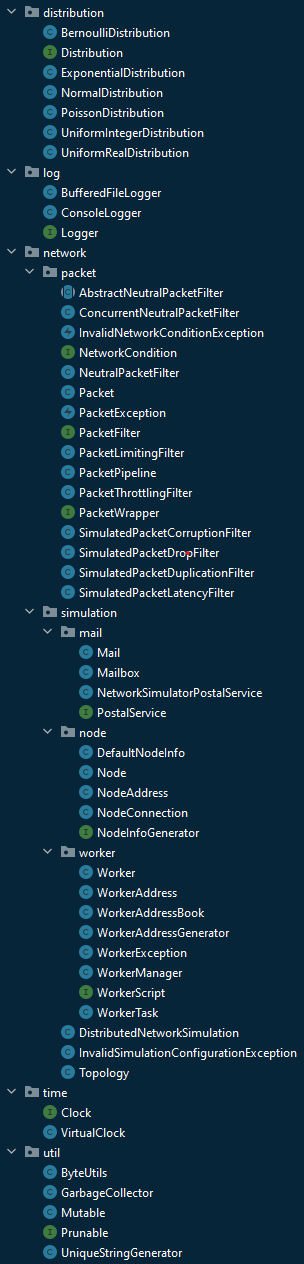
\includegraphics[width=0.35\textwidth]{images/interim_file_structure}
\end{center}

I currently don't have a name for the tool, but it has absolute parity with \texttt{tc-netem} (semantics which I'm
likely to change as the project evolves). Here is an example of some working setup code which one might write to
configure and run a simulation:

\begin{center}
    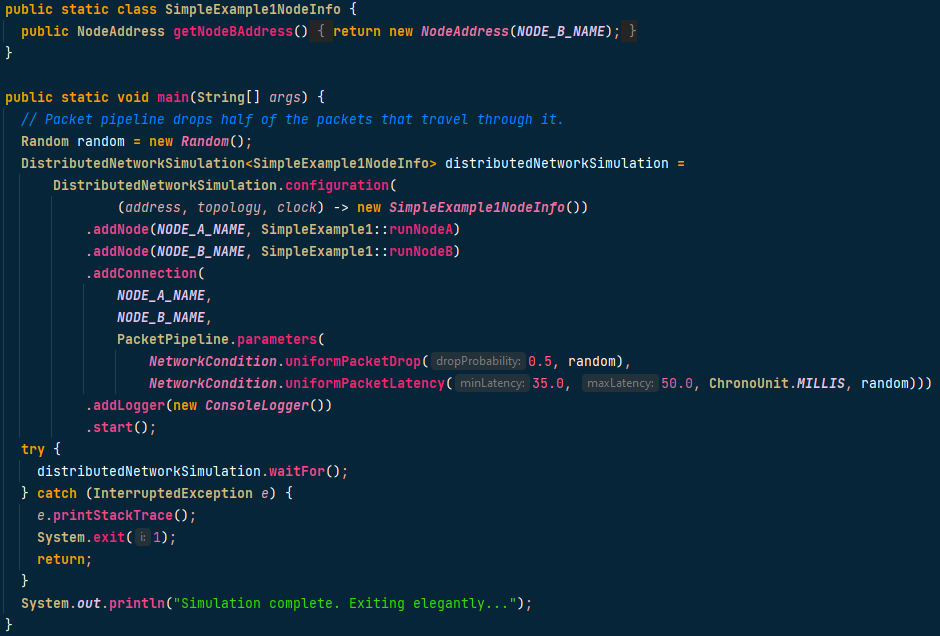
\includegraphics[width=\textwidth]{images/interim_example_sim_code}
\end{center}

A quick rundown on the current semantics. Nodes are connected in a topology. Each connection in said topology admits
of a packet pipeline, which applies a sequence of network conditions to packets which flow through it, i.e.:
probabilistic drop, corruption, duplication or latency, or perhaps even bandwidth throttling or packet limiting. Each
node runs one or more workers, which are essentially wrapped threads. Each worker has an address. Workers send
messages to other workers. These messages are routed by nodes. For example, if worker 1 running on node A sent a
message to worker 2 running on node B, this message would ultimately be serialized into a packet, go through the packet
pipeline connecting node A and node B. If this packet survives the trip, then node B will look up worker 2 in its
address book and post it to worker 2's mailbox (providing that worker 2 exists). For the purposes of simplicity, the
addressing mechanism is an artifact of the simulation logic, and cannot fall foul of corruption, i.e.: a message
addressed to worker 2 will only be delivered to worker 2, if it is delivered at all. If a user wishes to bake their
own custom addressing mechanism (that is fallible to corruption) into the provided framework, then they are free to
do so.

Nodes \texttt{A} and \texttt{B} are each given a \texttt{WorkerScript} during this setup, which are special kinds of
lambda. A \texttt{WorkerScript} is a function which takes a \texttt{WorkerManager} as a parameter, which in turn
provides each worker with a variety of important utilities, such as sending and receiving mail, or spawning child
workers.

I'm currently hosting the repository privately on GitHub and am using a Kanban board to organise and prioritise my work:

\begin{center}
    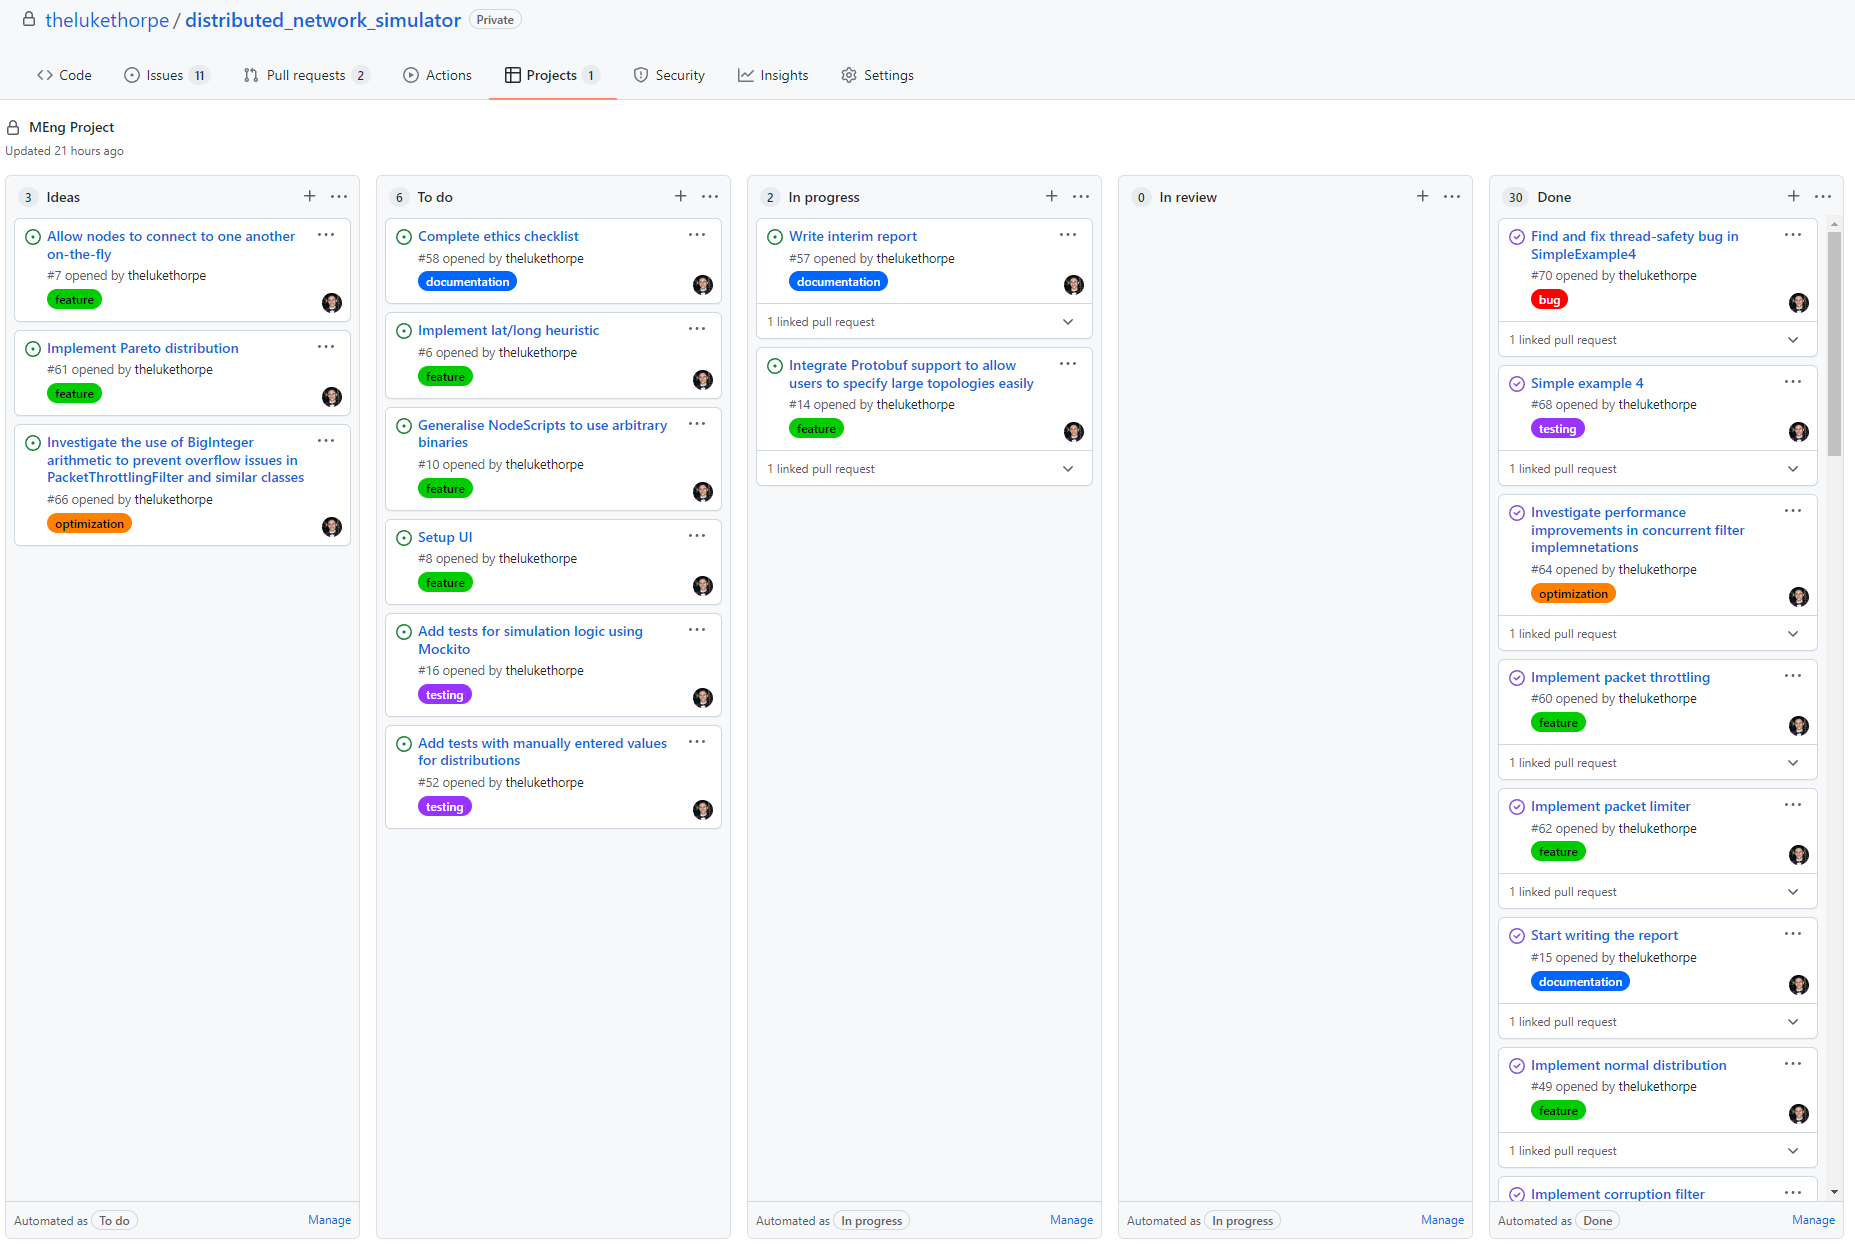
\includegraphics[width=\textwidth]{images/interim_kanban_board}
\end{center}

Thus, I'm looking to get the following work done by 1/4/22 [$\sim$10 university week budget with 1 week written-off for
exams]:
\begin{itemize}
    \item Come up with a good name for the tool (and the project as a whole) [<1 day].
    \item Research and writeup findings on 1 or 2 other simulation tools [$\sim$2 weeks].
    \item Research and writeup findings on Kubernetes, Docker, gRPC and Protobuf [$\sim$2 weeks].
    \item Research and writeup findings on 1 or 2 other pieces of related work [$\sim$2 weeks].
    \item Document semantics of the proposed solution as part of the Design section [$\sim$1 week].
    \item Implement Protobuf support to allow users to specify large topologies easily [$\sim$1 week].
    \item Investigate performance ramifications of current semantics and writeup findings [$\sim$1 week].
\end{itemize}


\section{INTERIM REPORT ONLY: Evaluation Plan}

TODO
